\chapter{Event-Driven Architecture}
\label{bab:event}

\section*{Tujuan Pembelajaran}

\begin{enumerate}
  \item Menjelaskan pembagian antara penerbit, event, dan pelanggan beserta
    kontrak yang menghubungkan ketiganya.
  \item Membedakan topologi broker dari topologi mediator, lalu menentukan
    kapan masing-masing layak dipilih.
  \item Mengukur \textit{latency cost}, \textit{failure containment}, dan
    \textit{change cost} pada ketiga susunan.
\end{enumerate}

\section{Pendahuluan}

Sebuah permintaan jarang berhenti pada satu pekerjaan. Satu permintaan konversi
kurs, misalnya, perlu dicatat ke riwayat, diperiksa nilainya, lalu
diberitahukan kepada pemohon. Cara paling lurus adalah memanggil ketiga
pekerjaan itu berurutan dari satu tempat. Cara itu bekerja, namun pemanggilnya
lalu terikat pada ketiga pekerjaan tersebut sekaligus.

\textit{Event-driven architecture} menawarkan ikatan yang lebih longgar.
Pemanggil cukup mengumumkan bahwa sesuatu telah terjadi, lalu berhenti di situ.
Pihak yang berkepentingan mendaftarkan diri sendiri, dan pengumuman itu
sampai kepada mereka tanpa disebut namanya. Bentuk pengumumannya disebut event,
yaitu catatan tentang sesuatu yang sudah terjadi, bukan perintah tentang
sesuatu yang harus dikerjakan.

Bab ini membandingkan tiga susunan yang mengerjakan pekerjaan sama persis,
yaitu panggilan berantai langsung, topologi broker, dan topologi mediator.
Kedua topologi berbasis event tersebut diambil dari kerangka yang disusun
Richards dan Ford~\cite{richards2020fundamentals}, sedangkan nama pola
\textit{message}-nya mengikuti katalog Hohpe dan Woolf~\cite{hohpe2003eip}.

\section{Penerbit, Event, dan Pelanggan}

Susunannya terdiri atas tiga peran. \textbf{Penerbit} mengumumkan bahwa sesuatu
telah terjadi, lalu selesai. \textbf{Event} adalah \textit{message} yang membawa kabar
tersebut beserta datanya. \textbf{Pelanggan} menyatakan minat pada satu jenis
kabar, lalu mengerjakan bagiannya setiap kali kabar itu datang.

Hohpe dan Woolf menyebut salurannya \textit{publish-subscribe
channel}~\cite{hohpe2003eip}. Saluran seperti itu mengirimkan satu salinan
kepada setiap pelanggan, sehingga penerbit tidak perlu tahu jumlah maupun nama
penerimanya. Gambar~\ref{fig:event-alur} menunjukkan bentuknya. Menambah kotak
baru di sisi kanan tidak menyentuh kotak di sisi kiri.

\begin{figure}[htbp]
  \centering
  \begin{tikzpicture}[
    kotak/.style={draw, rounded corners=2pt, minimum width=2.0cm,
      minimum height=0.9cm, align=center, font=\scriptsize\bfseries},
    panah/.style={-{Stealth[length=2mm]}, thick}
  ]
    \node[kotak, fill=gray!22] (penerbit) {Penerbit\\
      {\tiny\mdseries kirim()}};
    \node[kotak, fill=praditagreen!25, right=1.0cm of penerbit,
      minimum width=2.5cm] (topik) {Topik\\
      {\tiny\mdseries permintaan.diterima}};
    \node[kotak, fill=blue!8, above right=0.45cm and 1.0cm of topik] (p1)
      {Pencatat};
    \node[kotak, fill=blue!8, right=1.0cm of topik] (p2) {Pemeriksa};
    \node[kotak, fill=green!10, below right=0.45cm and 1.0cm of topik] (p3)
      {Pelanggan baru};

    \draw[panah] (penerbit) -- node[above, font=\tiny] {event} (topik);
    \draw[panah] (topik) -- (p1);
    \draw[panah] (topik) -- (p2);
    \draw[panah] (topik) -- (p3);
  \end{tikzpicture}
  \caption{Penerbit hanya mengenal nama topik. Pelanggan mendaftarkan dirinya
    sendiri, sehingga kotak baru dapat muncul tanpa mengubah penerbitnya}
  \label{fig:event-alur}
\end{figure}

Analogi yang mendekati adalah pengumuman lewat pengeras suara kampus. Petugas
membacakan bahwa jadwal ujian sudah terbit, lalu meletakkan mikrofonnya.
Petugas itu tidak menghubungi satu per satu mahasiswa, dan tidak menunggu
satu pun tanggapan. Mahasiswa yang berkepentingan mendengar lalu mengerjakan
urusannya masing-masing, sedangkan yang sedang berada di luar gedung tidak
mendengar apa pun. Pengumuman yang sudah dibacakan juga tidak dapat ditarik
kembali.

Pembagian ketiga peran tersebut menentukan letak setiap keputusan.
Tabel~\ref{tab:peran-event} merangkum tanggung jawab dan larangan masing-masing.

\begin{table}[htbp]
  \centering
  \caption{Tanggung jawab dan larangan penerbit, event, serta pelanggan}
  \label{tab:peran-event}
  \begin{tabularx}{\textwidth}{|l|X|X|}
    \hline
    \textbf{Peran} & \textbf{Tanggung jawab} & \textbf{Tidak boleh mengetahui} \\
    \hline
    Penerbit & Mengumumkan kabar beserta datanya pada satu topik & Nama, jumlah, dan nasib pelanggan mana pun \\
    \hline
    Event & Membawa kabar yang sudah terjadi, bukan perintah & Cara pelanggan mengerjakan bagiannya \\
    \hline
    Pelanggan & Mengerjakan satu bagian setiap kali kabarnya datang & Nama pelanggan lain pada topik yang sama \\
    \hline
  \end{tabularx}
\end{table}

Satu kalimat pada tabel tersebut sering terlewat, yaitu event membawa kabar,
bukan perintah. Perbedaannya terlihat pada penamaannya. Nama
\texttt{permintaan.dicatat} menyebut sesuatu yang sudah terjadi, sedangkan nama
\texttt{catat\_permintaan} menyebut sesuatu yang harus dikerjakan. Nama kedua
memaksa penerbit tahu bahwa ada pihak yang mencatat, dan ikatan itulah yang
sebenarnya hendak dilepas.

\section{Topologi Broker}

Pertanyaan berikutnya menyusul dengan sendirinya. Bila penerbit tidak mengatur
siapa pun, siapa yang menentukan urutan langkahnya. Jawaban pertama adalah
tidak ada yang menentukan, dan susunan itulah yang disebut \textbf{topologi
broker}.

Pada topologi broker, setiap pelanggan mengerjakan bagiannya lalu menerbitkan
event baru tentang apa yang baru saja dikerjakannya. Pelanggan berikutnya
mendengar event itu, bekerja, lalu menerbitkan event berikutnya lagi. Urutan
langkah karena itu tidak tertulis di satu tempat, melainkan tersebar pada
pilihan topik setiap pelanggan. Richards dan Ford menggambarkannya sebagai
aliran \textit{message} berantai tanpa pengatur pusat~\cite{richards2020fundamentals}.

Gambar~\ref{fig:rantai-broker} menunjukkan rantai pada contoh bab ini. Tiga
event terbit untuk satu permintaan, dan tidak satu pun kotak menyebut nama
kotak sesudahnya.

\begin{figure}[htbp]
  \centering
  \begin{tikzpicture}[
    kotak/.style={draw, rounded corners=2pt, minimum width=2.6cm,
      minimum height=0.8cm, align=center, font=\scriptsize\bfseries},
    panah/.style={-{Stealth[length=2mm]}, thick}
  ]
    \node[kotak, fill=gray!22] (penerbit) {Penerbit};
    \node[kotak, fill=blue!8, below=0.85cm of penerbit] (catat) {Pencatat};
    \node[kotak, fill=blue!8, below=0.85cm of catat] (periksa) {Pemeriksa};
    \node[kotak, fill=green!10, below=0.85cm of periksa] (beritahu)
      {Pemberitahu};

    \draw[panah] (penerbit) -- node[right, font=\tiny]
      {\texttt{permintaan.diterima}} (catat);
    \draw[panah] (catat) -- node[right, font=\tiny]
      {\texttt{permintaan.dicatat}} (periksa);
    \draw[panah] (periksa) -- node[right, font=\tiny]
      {\texttt{permintaan.diperiksa}} (beritahu);
  \end{tikzpicture}
  \caption{Rantai pada topologi broker. Setiap pelanggan menerbitkan kabar
    tentang pekerjaannya sendiri, lalu berhenti tanpa tahu siapa yang
    mendengarnya}
  \label{fig:rantai-broker}
\end{figure}

Brokernya sendiri kecil. Yang disimpannya hanya pasangan antara nama topik dan
daftar antrean pelanggannya, sehingga menerbitkan berarti menaruh satu salinan
pada setiap antrean. Listing~\ref{lst:langganan} memperlihatkan kedua
fungsinya.

\begin{lstlisting}[style=PythonStyle, caption={Inti broker, tersedia di
  \berkas{sources/chapter09/broker.py}}, label=lst:langganan]
def langganan(self, topik: str, penangan) -> queue.Queue:
  """Mendaftarkan satu pelanggan pada satu topik beserta threadnya."""
  antrean = queue.Queue()
  self.langganan_topik.setdefault(topik, []).append(antrean)
  utas = threading.Thread(target=self.layani, daemon=True,
                          args=(topik, antrean, penangan))
  utas.start()
  self.thread.append((antrean, utas))
  return antrean


def terbitkan(self, topik: str, pesan: domain.Permintaan) -> int:
  """Menaruh pesan pada antrean setiap pelanggan topik tersebut."""
  antrean_pelanggan = self.langganan_topik.get(topik, [])
  for antrean in antrean_pelanggan:
    antrean.put(pesan)
  with self.kunci:
    self.jumlah_pesan += len(antrean_pelanggan)
  return len(antrean_pelanggan)
\end{lstlisting}

Rantainya pun sependek itu. Setiap penangan memanggil satu pemroses, lalu
menerbitkan kabar tentang pekerjaan yang baru saja selesai.

\begin{lstlisting}[style=PythonStyle, caption={Rantai pelanggan pada topologi
  broker, tersedia di \berkas{sources/chapter09/broker.py}}, label=lst:rantai]
def saat_diterima(self, permintaan: domain.Permintaan) -> None:
  """Mencatat permintaan, lalu mengumumkan bahwa pencatatannya selesai."""
  self.pencatat.tangani(permintaan)
  self.broker.terbitkan(TOPIK_DICATAT, permintaan)


def saat_dicatat(self, permintaan: domain.Permintaan) -> None:
  """Memeriksa permintaan, lalu mengumumkan bahwa pemeriksaannya selesai."""
  self.pemeriksa.tangani(permintaan)
  self.broker.terbitkan(TOPIK_DIPERIKSA, permintaan)
\end{lstlisting}

Broker pada bab ini dibuat dari \texttt{queue.Queue} dan \textit{thread}
pustaka standar Python, sehingga seluruh latihan berjalan pada satu laptop.
Broker sungguhan menambahkan beberapa hal yang tidak dimiliki antrean dalam
memori. Kafka, misalnya, menyimpan setiap event ke cakram dalam urutan yang
tetap, menahannya selama tenggat yang diatur, lalu membiarkan pelanggan
membacanya ulang dari posisi yang dicatat sendiri~\cite{kafka2026docs}. Bentuk
berlangganannya tetap sama, dan itulah yang dipelajari di sini.

Gambar~\ref{fig:kelas-event} menunjukkan hubungan kelasnya. Perhatikan bahwa
tidak ada satu pun panah yang berangkat dari broker menuju pemroses.

\begin{figure}[htbp]
  \centering
  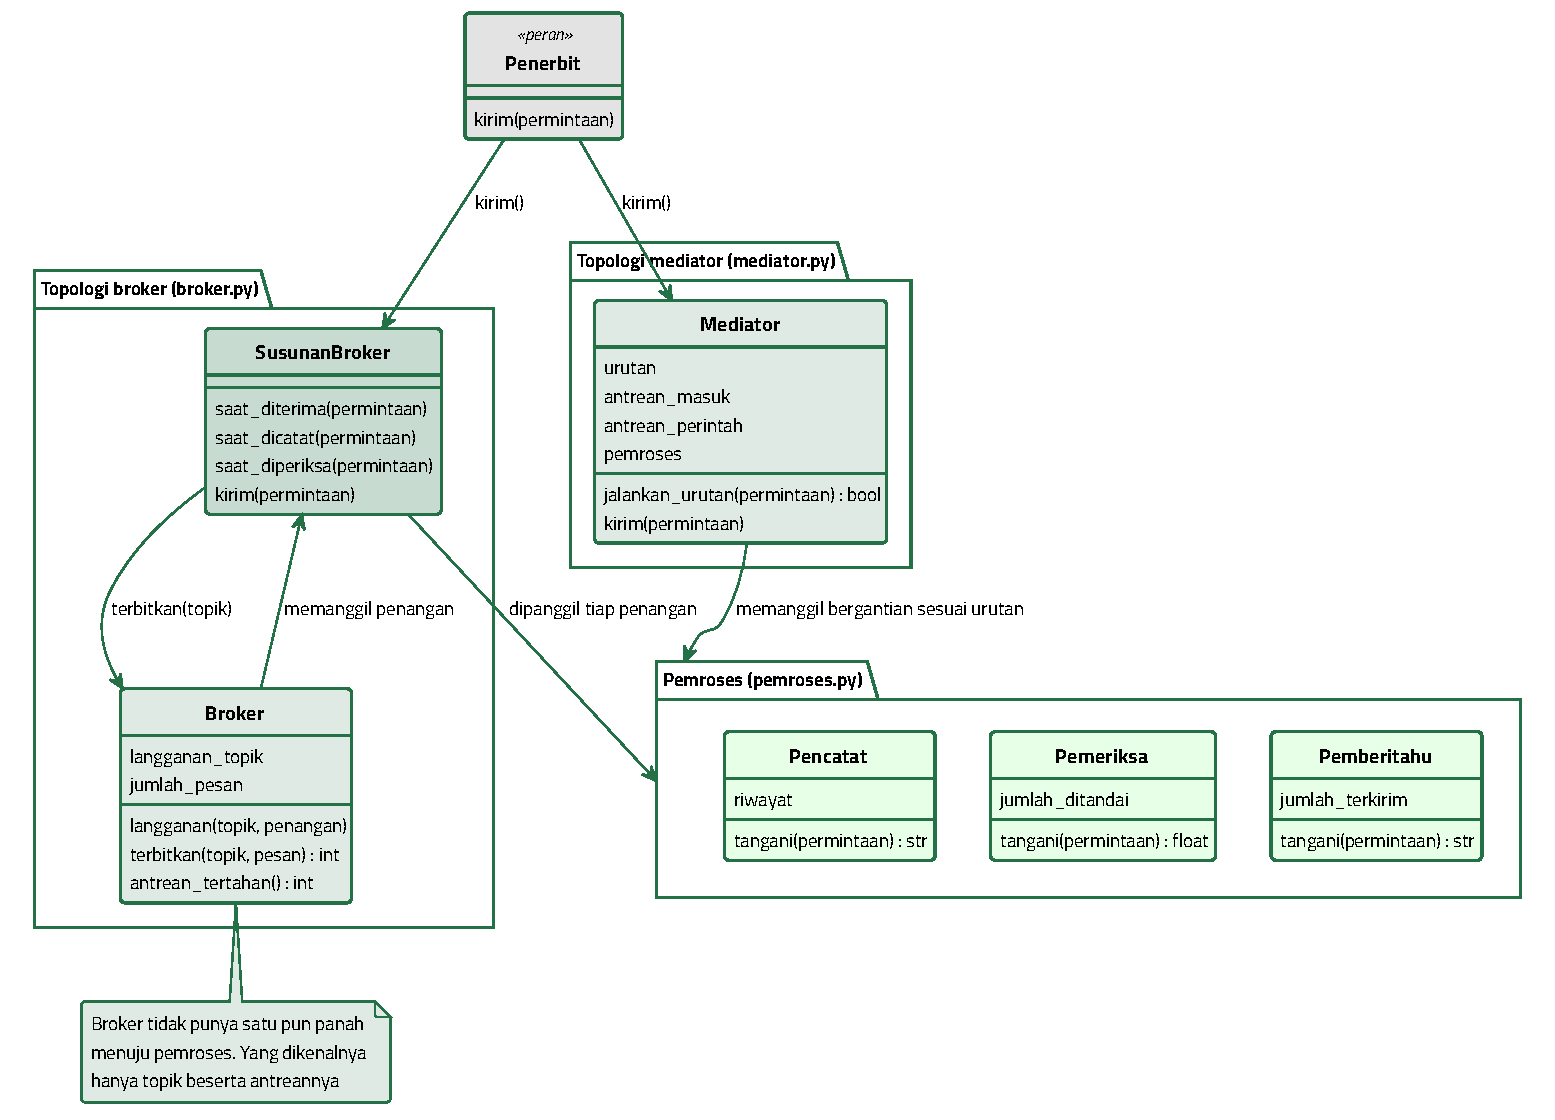
\includegraphics[width=\textwidth, height=0.44\textheight,
    keepaspectratio]{kelas-event.pdf}
  \caption{Broker hanya mengenal topik beserta antreannya, sedangkan mediator
    menyimpan rujukan ke setiap pemroses yang urutannya dipegangnya}
  \label{fig:kelas-event}
\end{figure}

\section{Topologi Mediator}

Kelonggaran tersebut membawa kerugian yang segera terasa. Bila urutan langkah
tersebar pada pilihan topik, tidak ada satu tempat pun yang dapat ditanyai
tentang keseluruhan alurnya. Pertanyaannya, bagaimana bila urutan itu justru
perlu dipegang seseorang.

Jawabannya adalah \textbf{topologi mediator}. Penerbit mengirim permintaan ke
satu pengatur, dan pengatur itulah yang memegang daftar langkahnya. Pengatur
memanggil pemroses pertama, menunggu balasannya, lalu memanggil pemroses kedua.
Karena menunggu, pengatur tahu persis langkah mana yang gagal dan langkah mana
yang belum sempat dijalankan.

Analoginya adalah ketua panitia wisuda. Ketua memegang susunan acara, menelepon
seksi konsumsi, menunggu laporan selesai, baru menelepon seksi dekorasi. Bila
seksi konsumsi melapor gagal, ketua tahu acara berhenti di \textit{identifier} itu dan tahu
seksi mana yang belum dihubungi. Harganya adalah setiap kabar melewati satu
orang yang sama, dan orang itu hanya dapat menangani satu urusan pada satu
waktu.

Gambar~\ref{fig:bintang-mediator} menunjukkan bentuknya. Setiap langkah
terdiri atas satu perintah dan satu balasan.

\begin{figure}[htbp]
  \centering
  \begin{tikzpicture}[
    kotak/.style={draw, rounded corners=2pt, minimum width=2.0cm,
      minimum height=0.8cm, align=center, font=\scriptsize\bfseries},
    panah/.style={-{Stealth[length=2mm]}, thick},
    balasan/.style={-{Stealth[length=2mm]}, thick, dashed}
  ]
    \node[kotak, fill=gray!22] (penerbit) {Penerbit};
    \node[kotak, fill=praditagreen!25, right=1.3cm of penerbit,
      minimum height=1.5cm] (mediator) {Mediator\\
      {\tiny\mdseries urutan langkah}};
    \node[kotak, fill=blue!8, right=2.0cm of mediator] (periksa) {Pemeriksa};
    \node[kotak, fill=blue!8, above=0.45cm of periksa] (catat) {Pencatat};
    \node[kotak, fill=green!10, below=0.45cm of periksa] (beritahu)
      {Pemberitahu};

    \draw[panah] (penerbit) -- node[above, font=\tiny] {masuk} (mediator);
    \draw[panah] (mediator.east) -- node[above, font=\tiny, pos=0.6]
      {perintah} (catat.west);
    \draw[panah] (mediator.east) -- (periksa.west);
    \draw[panah] (mediator.east) -- (beritahu.west);
    \draw[balasan] (periksa.west) to[bend left=22]
      node[below, font=\tiny, pos=0.5] {balasan} (mediator.east);
  \end{tikzpicture}
  \caption{Mediator memegang urutan langkah. Setiap pemroses dipanggil
    bergantian, dan balasannya ditunggu sebelum langkah berikutnya dimulai}
  \label{fig:bintang-mediator}
\end{figure}

Isi pengaturnya hanya satu perulangan. Listing~\ref{lst:urutan}
memperlihatkannya, termasuk apa yang dicatat ketika satu langkah gagal.

\begin{lstlisting}[style=PythonStyle, caption={Urutan langkah pada mediator,
  tersedia di \berkas{sources/chapter09/mediator.py}}, label=lst:urutan]
def jalankan_urutan(self, permintaan: domain.Permintaan) -> bool:
  """Memanggil setiap pemroses bergantian, lalu berhenti pada galat pertama."""
  for nomor_langkah, nama in enumerate(self.urutan):
    self.antrean_perintah[nama].put(permintaan)
    self.hitung_pesan(1)
    _, _, galat = self.antrean_balasan.get()
    if galat is not None:
      sisa = self.urutan[nomor_langkah + 1:]
      self.gagal.append((permintaan.nomor, nama, list(sisa)))
      return False
  return True
\end{lstlisting}

Gambar~\ref{fig:sekuens-event} membandingkan satu permintaan pada kedua
topologi. Jumlah \textit{message}-nya berbeda, dan selisih itu bukan kebetulan.

\begin{figure}[htbp]
  \centering
  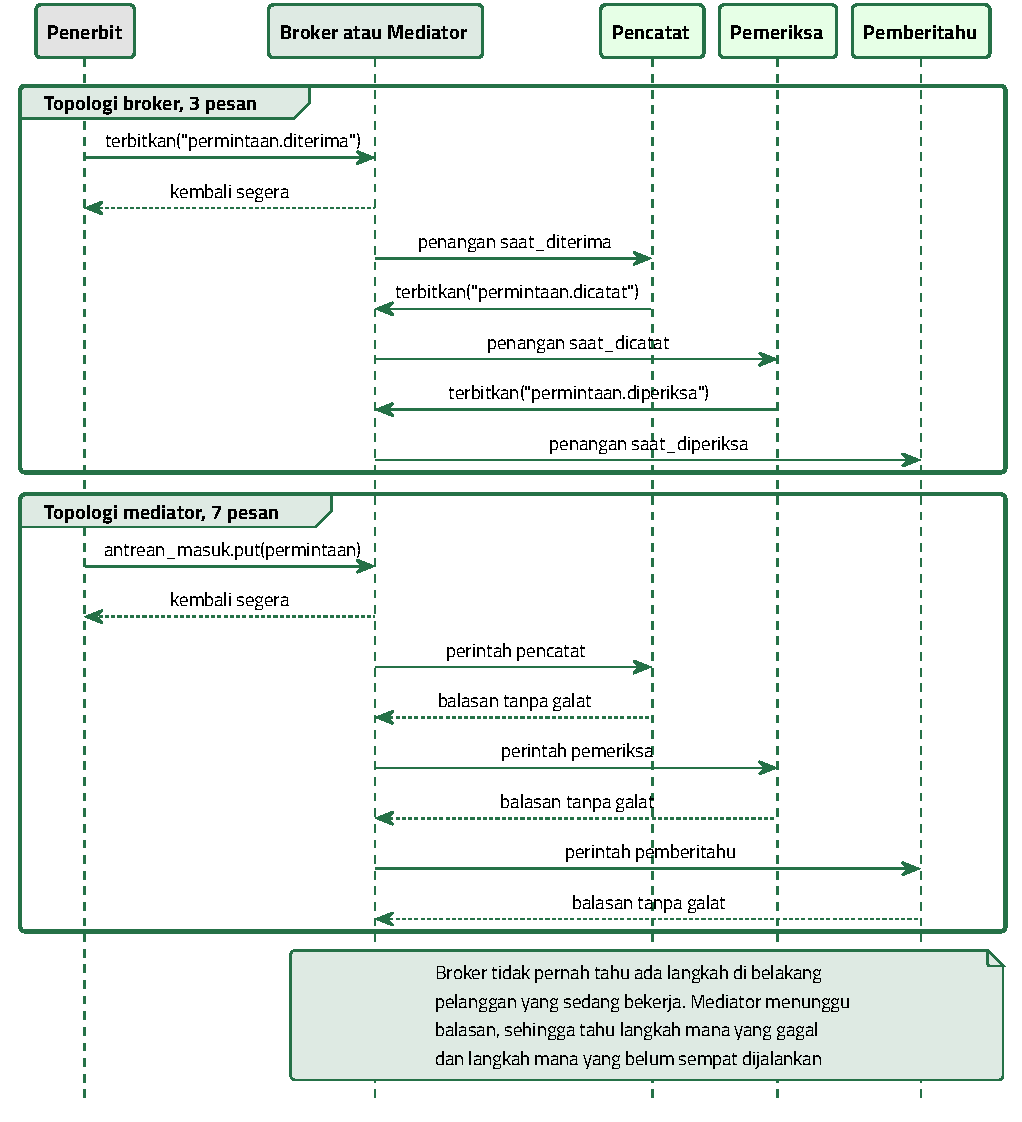
\includegraphics[width=0.86\textwidth, height=0.52\textheight,
    keepaspectratio]{sekuens-event.pdf}
  \caption{Satu permintaan menempuh tiga \textit{message} pada topologi broker dan tujuh
    \textit{message} pada topologi mediator, sebab setiap langkah mediator berupa perintah
    beserta balasannya}
  \label{fig:sekuens-event}
\end{figure}

Selisih jumlah \textit{message} itulah harga pengawasan terpusat.
Tabel~\ref{tab:jumlah-pesan} merinci asalnya pada ketiga susunan, dan angkanya
dihitung skrip, bukan ditaksir.

\begin{table}[htbp]
  \centering
  \caption{Jumlah \textit{message} yang melewati antrean untuk satu permintaan}
  \label{tab:jumlah-pesan}
  \begin{tabularx}{\textwidth}{|l|l|X|}
    \hline
    \textbf{Susunan} & \textbf{\textit{Message}} & \textbf{Rinciannya} \\
    \hline
    Sinkron & 0 & Ketiga langkah berupa pemanggilan langsung di dalam satu \textit{thread} \\
    \hline
    Broker & 3 & Satu event per langkah, masing-masing menuju satu pelanggan \\
    \hline
    Mediator & 7 & Satu \textit{message} masuk, ditambah satu perintah dan satu balasan per langkah \\
    \hline
  \end{tabularx}
\end{table}

\section{Harga Satu Permintaan}

Ketiga susunan mengerjakan pekerjaan yang sama persis, sebab ketiganya memanggil
kelas pemroses yang sama dari \berkas{sources/chapter09/pemroses.py}. Karena itu
selisih waktunya hanya berasal dari cara \textit{message}-nya disampaikan. Skrip
\texttt{ukur\_latensi.py} menjalankan dua ratus putaran, dan ketiga susunan
diukur berselang-seling di dalam putaran yang sama agar beban mesin yang
berubah menimpa ketiganya sekaligus.

Dua waktu dicatat pada setiap permintaan. Waktu penerbit kembali dihitung
sampai fungsi \texttt{kirim} kembali, sedangkan latensi ujung ke ujung dihitung
sampai langkah terakhir selesai. Tabel~\ref{tab:latensi} memuat hasilnya.

\begin{table}[htbp]
  \centering
  \caption{Latensi ketiga susunan pada dua ratus permintaan, dalam milidetik}
  \label{tab:latensi}
  \begin{tabularx}{\textwidth}{|l|l|l|l|l|X|}
    \hline
    \textbf{Susunan} & \textbf{Median} & \textbf{P95} & \textbf{Terbesar} & \textbf{Kembali} & \textbf{\textit{Message}} \\
    \hline
    Sinkron & 0,0065 & 0,0108 & 0,0230 & 0,0059 & 0 \\
    \hline
    Broker & 0,0361 & 0,0600 & 0,0730 & 0,0029 & 3 \\
    \hline
    Mediator & 0,0544 & 0,0725 & 0,1129 & 0,0025 & 7 \\
    \hline
  \end{tabularx}
\end{table}

Angka tersebut menolak satu harapan yang sering dibawa ke bab ini, yaitu bahwa
event membuat permintaan lebih cepat. Median susunan broker 5,5 kali median
susunan sinkron, dan susunan mediator 8,3 kali. Selisihnya pun bukan kebetulan.
\textit{Range} di dalam jalur sinkron tercatat 0,0177 milidetik, sedangkan
selisih median terhadap broker 0,0296 milidetik, yaitu 1,7 kali
\textit{range} itu. Pencacahan per putaran menegaskannya, yaitu susunan sinkron
lebih cepat pada 200 dari 200 putaran.

Sebabnya terletak pada perpindahan antar \textit{thread}. Setiap \textit{message} yang
masuk antrean harus membangunkan \textit{thread} lain, dan pembangunan itu
jauh lebih mahal daripada pekerjaan yang diangkutnya. Pekerjaan pada bab ini
memang sangat kecil, yaitu satu perkalian dan dua penyusunan teks, sehingga
\textit{cost} pengangkutannya justru mendominasi.

Kolom kembali memuat kejanggalan yang perlu dibaca hati-hati. Susunan broker
kembali 0,0030 milidetik lebih cepat daripada susunan sinkron, padahal
\textit{range} di dalam jalur sinkron 5,9 kali lebih besar daripada selisih
itu. Menurut ukuran Bab~2, selisih sekecil itu belum dapat disebut ada.
Pencacahan per putaran justru menunjuk arah yang jelas, yaitu susunan berbasis
event kembali lebih cepat pada 199 dari 200 putaran. Sebagaimana pada Bab~6,
pencacahan lebih peka daripada median, sebab median menyerap satu putaran
lambat sebagai angka besar sedangkan pencacahan hanya melihat siapa yang
menang.

Selisih sekecil itu memang tidak menarik. Yang menarik adalah apa yang terjadi
pada selisih tersebut ketika satu pemroses mulai lambat, dan seksi berikutnya
mengukurnya.

\section{Ketika Satu Pemroses Tersendat}

Kasus berikut memperlihatkan taruhannya. Sebuah loket pembayaran uang kuliah
memakai susunan sinkron. Setiap pembayaran dicatat, diperiksa, lalu
diberitahukan lewat layanan \textit{message} singkat milik pihak ketiga. Pada hari biasa
layanan itu menjawab dalam puluhan milidetik. Pada hari terakhir pembayaran,
layanan tersebut tersendat dan jawabannya berubah menjadi lima detik. Petugas
loket tidak dapat menerima pembayaran berikutnya sebelum jawaban itu datang,
antrean mahasiswa mengular, dan sebagian pulang tanpa membayar. Pencatatan dan
pemeriksaannya sendiri sebenarnya sudah selesai sejak awal.

Skrip \texttt{uji\_ketahanan.py} menjalankan dua skenario atas cerita tersebut.
Skenario pertama memasang pemeriksa yang menolak setiap permintaan kelipatan
lima. Tabel~\ref{tab:gagal} memuat hasilnya atas seratus permintaan.

\begin{table}[htbp]
  \centering
  \caption{Nasib seratus permintaan ketika pemeriksa gagal berkala}
  \label{tab:gagal}
  \begin{tabularx}{\textwidth}{|l|l|l|l|l|X|}
    \hline
    \textbf{Susunan} & \textbf{Tuntas} & \textbf{Tercatat} & \textbf{Diberitahu} & \textbf{Galat} & \textbf{Berhenti} \\
    \hline
    Sinkron & 4 & 5 & 4 & 0 & pada nomor 5 \\
    \hline
    Broker & 80 & 100 & 80 & 20 & tidak \\
    \hline
    Mediator & 80 & 100 & 80 & 20 & tidak \\
    \hline
  \end{tabularx}
\end{table}

Baris pertama itulah yang paling tajam. Susunan sinkron berhenti pada
permintaan kelima, sehingga sembilan puluh lima permintaan sesudahnya tidak
pernah tersentuh. Kedua susunan berbasis event menampung galatnya di dalam
\textit{thread} pelanggan, sehingga delapan puluh permintaan tetap tuntas dan
seluruh seratus permintaan tetap tercatat.

Kedua susunan berbasis event menghasilkan angka yang sama, namun catatan
galatnya berbeda. Broker mencatat topik beserta nomor permintaannya, yaitu
\texttt{topik permintaan.dicatat, permintaan 5}. Mediator mencatat langkah yang
gagal sekaligus sisa langkah yang belum dijalankan, yaitu \texttt{permintaan 5
putus pada pemeriksa, sisa ['pemberitahu']}. Hanya mediator yang memegang
urutan lengkapnya, sehingga hanya mediator yang dapat mengulang sisa langkah
itu kelak.

Skenario kedua memasang pemeriksa yang menahan setiap permintaan selama lima
milidetik. Tabel~\ref{tab:lambat} memuat hasilnya, dan seluruh waktunya
dihitung untuk seratus permintaan sekaligus, bukan per permintaan.

\begin{table}[htbp]
  \centering
  \caption{Seratus permintaan ketika pemeriksa menahan lima milidetik}
  \label{tab:lambat}
  \begin{tabularx}{\textwidth}{|l|l|l|l|X|}
    \hline
    \textbf{Susunan} & \textbf{Penerbit kembali} & \textbf{Antrean terdalam} & \textbf{Seluruh tercatat} & \textbf{Seluruh tuntas} \\
    \hline
    Sinkron & 517,6 ms & 0 & 518,0 ms & 518,2 ms \\
    \hline
    Broker & 0,4 ms & 100 & 1,9 ms & 518,4 ms \\
    \hline
    Mediator & 0,4 ms & 100 & 543,7 ms & 548,2 ms \\
    \hline
  \end{tabularx}
\end{table}

Di sinilah selisih yang tadi tenggelam berubah menjadi besar. Penerbit pada
susunan sinkron tertahan 517,6 milidetik, sedangkan penerbit pada kedua susunan
berbasis event kembali sesudah 0,4 milidetik. Perbandingannya lebih dari seribu
kali, dan besarnya persis sebanding dengan lamanya pemroses tersendat.
Itulah yang sebenarnya dibeli dengan tambahan \textit{message} pada seksi sebelumnya.

Kolom antrean terdalam memuat harga yang menyertainya. Pekerjaan yang tidak
lagi ditunggu penerbit tidak lenyap, melainkan menumpuk, dan puncaknya seratus
\textit{message} pada kedua susunan berbasis event. Susunan sinkron tidak punya tumpukan
sama sekali, sebab tekanannya langsung dirasakan penerbit sebagai waktu tunggu.
Antrean yang menumpuk itu harus dipantau, sebab antrean yang tumbuh lebih cepat
daripada pemrosesnya akan menghabiskan memori.

Kolom seluruh tercatat memisahkan kedua topologi berbasis event.
Seratus permintaan selesai dicatat sesudah 1,9 milidetik pada topologi broker,
sedangkan topologi mediator membutuhkan 543,7 milidetik untuk pekerjaan yang
sama. Sebabnya, pencatat pada topologi broker punya antrean sendiri dan tidak
menunggu pemeriksa, sedangkan mediator menangani satu permintaan pada satu
waktu sehingga langkah pertama permintaan kedua baru mulai sesudah permintaan
pertama tuntas. Pengawasan terpusat karena itu bukan hanya menambah \textit{message},
melainkan juga membuat pengaturnya menjadi leher botol.

\section{Biaya Menambah Pelanggan}

Ukuran terakhir bab ini adalah biaya perubahan. Bagian audit meminta setiap
permintaan disalin ke jurnal tersendiri, sehingga satu pemroses baru harus
disisipkan. Direktori \berkas{sources/chapter09/varian_audit/} memuat ketiga
berkas susunan sesudah penyisipan itu, dan skrip \texttt{ukur\_perubahan.py}
menghitung selisih barisnya. Baris kosong, baris komentar, dan docstring modul
dilewati, sebab ketiganya tidak menentukan perilaku program.

Tabel~\ref{tab:perubahan} memuat hasilnya. Berkas barunya sama bagi ketiga
susunan, yaitu satu berkas \texttt{audit.py}.

\begin{table}[htbp]
  \centering
  \caption{Biaya menyisipkan satu pemroses baru pada ketiga susunan}
  \label{tab:perubahan}
  \begin{tabularx}{\textwidth}{|l|l|l|l|X|}
    \hline
    \textbf{Susunan} & \textbf{Baris tambah} & \textbf{Baris hapus} & \textbf{\textit{Message} sebelum} & \textbf{\textit{Message} sesudah} \\
    \hline
    Sinkron & 6 & 3 & 0 & 0 \\
    \hline
    Broker & 3 & 0 & 3 & 4 \\
    \hline
    Mediator & 3 & 1 & 7 & 9 \\
    \hline
  \end{tabularx}
\end{table}

Selisih angkanya kecil, dan kekecilan itu jujur. Yang lebih menentukan adalah
letak barisnya. Pada susunan sinkron, baris baru masuk ke dalam badan
\texttt{kirim}, yaitu alur bisnis yang dijalankan pada setiap permintaan. Pada
topologi broker, baris baru hanya masuk ke bagian perakitan, sebab pelanggan
baru cukup berlangganan pada topik yang sudah ada. Pada topologi mediator,
baris baru masuk ke bagian perakitan sekaligus ke daftar urutan langkah, sebab
mediator hanya menjalankan langkah yang tercantum di sana.

Kolom \textit{message} memuat biaya yang terus berjalan sesudah perubahan itu. Pelanggan
baru menambah satu \textit{message} per permintaan pada topologi broker, dan dua \textit{message} per
permintaan pada topologi mediator. Selisih itu berulang pada setiap permintaan,
sedangkan selisih baris hanya dibayar sekali.

Satu kejanggalan muncul pada jejak langkahnya. Pada topologi mediator, jejaknya
selalu \texttt{pencatat, pemeriksa, pemberitahu, audit}, sedangkan pada topologi
broker jejaknya berubah-ubah. Dua belas kali penjalanan menghasilkan tiga
bentuk, yaitu \texttt{audit} di urutan pertama delapan kali, \texttt{audit} di
urutan terakhir tiga kali, dan \texttt{audit} di urutan kedua satu kali.
Sebabnya, pencatat audit berlangganan pada topik yang sama dengan pencatat
biasa, sehingga
keduanya berjalan sejajar di \textit{thread} masing-masing dan urutannya
ditentukan penjadwal sistem operasi. Kelonggaran itu memang yang diminta,
namun akibatnya urutan antar pelanggan sebuah topik tidak boleh diandalkan.

\section{\textit{Summary}}

\textit{Event-driven architecture} melepaskan penerbit dari nasib pihak yang
mengerjakan lanjutannya. Penerbit mengumumkan bahwa sesuatu telah terjadi, lalu
berhenti di situ. Pelanggan mendaftarkan dirinya sendiri pada topik yang
diminatinya, sehingga penerbit tidak pernah menyebut satu nama pun.

Kelonggaran tersebut dibayar dengan waktu. Pada contoh bab ini, latensi ujung
ke ujung topologi broker 5,5 kali latensi susunan sinkron, dan topologi mediator
8,3 kali. Susunan sinkron menang pada 200 dari 200 putaran, sebab perpindahan
antar \textit{thread} jauh lebih mahal daripada pekerjaan kecil yang
diangkutnya. Event karena itu tidak mempercepat satu permintaan.

Yang dibeli terlihat ketika satu pemroses tersendat. Pemeriksa yang menahan
lima milidetik membuat penerbit sinkron tertahan 517,6 milidetik untuk seratus
permintaan, sedangkan penerbit pada kedua susunan berbasis event kembali
sesudah 0,4 milidetik. Pemeriksa yang gagal berkala menghentikan susunan
sinkron pada permintaan kelima, sedangkan kedua susunan berbasis event tetap
menuntaskan delapan puluh permintaan dan mencatat seluruh seratus permintaan.

Pilihan antara kedua topologi berbasis event adalah pilihan antara kelonggaran
dan pengawasan. Topologi broker memakai tiga \textit{message} per permintaan, membiarkan
langkah pertama berjalan lepas dari langkah lambat di belakangnya, dan menerima
pelanggan baru tanpa menyentuh satu penangan lama pun. Topologi mediator
memakai tujuh \textit{message}, menahan permintaan berikutnya sampai yang sekarang tuntas,
namun tahu persis langkah mana yang putus beserta sisanya.

\textit{Message} utama bab ini karena itu bukan bahwa event membuat sistem lebih cepat,
melainkan bahwa event memindahkan waktu tunggu dari penerbit ke antrean.
Antrean itu terlihat pada angka, yaitu seratus \textit{message} yang menumpuk, dan angka
itulah yang harus dipantau ketika susunan berbasis event dipilih.

\section{Latihan}

Ketiga latihan berikut memakai satu basis kode yang sama di
\berkas{sources/chapter09/}, tetapi menyasar tiga masalah yang berbeda.
Latihan~1 mengukur \textit{latency cost}. Latihan~2 mengukur
\textit{failure containment} ketika satu pemroses gagal lalu lambat.
Latihan~3 menghitung \textit{change cost} saat satu pelanggan baru
ditambahkan.
Hasil setiap mahasiswa dapat berbeda, dan yang dilaporkan adalah pola
perbandingannya, bukan angka mutlaknya.

Venv yang sama dipakai kembali, dan pengaktifannya seperti pada
Listing~\ref{lst:venv-ch09}. Bab ini hanya memakai pustaka standar Python,
sehingga tidak ada pemasangan tambahan.

\begin{lstlisting}[language=bash, caption={Menyiapkan bahan sebelum ketiga
  latihan, seluruh skrip tersedia di \berkas{sources/chapter09/}},
  label=lst:venv-ch09]
bash sources/siapkan_venv.sh
source .venv/bin/activate
cd sources/chapter09
python sinkron.py
# Keluarannya baris kedua: Pesan lewat antrean: 0
python broker.py
# Keluarannya baris kedua: Pesan lewat antrean: 3
python mediator.py
# Keluarannya baris kedua: Pesan lewat antrean: 7
\end{lstlisting}

\subsection*{Latihan 1: \textit{Latency Cost}}

Latihan ini menguji harapan yang paling sering dibawa ke arsitektur berbasis
event, yaitu bahwa event membuat permintaan lebih cepat. Harapan itu menyebut
angka, sehingga dapat dibuktikan salah. Langkah kerjanya sebagai berikut.

\begin{enumerate}
  \item Jalankan perintah pada Listing~\ref{lst:jalankan-latensi}, lalu catat
    keenam angka pada baris ringkasan ketiga susunan.
  \item Catat pula \textit{range} jalur sinkron, selisih median, dan pencacahan
    putaran pada bagian perbandingannya.
  \item Buka \berkas{sources/chapter09/mediator.py}, lalu hitung sendiri asal
    angka tujuh \textit{message} per permintaan.
  \item Ubah \texttt{JUMLAH\_PERMINTAAN} menjadi lima ratus, jalankan ulang,
    lalu catat perubahan persentil ke-95 dan nilai terbesarnya.
\end{enumerate}

\begin{lstlisting}[language=bash, caption={Mengukur \textit{latency cost},
  skrip tersedia di \berkas{sources/chapter09/ukur_latensi.py}},
  label=lst:jalankan-latensi]
python ukur_latensi.py
# Keluarannya: sinkron   0.0065 ms  p95 0.0108  terbesar 0.0230  pesan 0
#              broker    0.0361 ms  p95 0.0600  terbesar 0.0730  pesan 3
#              mediator  0.0544 ms  p95 0.0725  terbesar 0.1129  pesan 7
#              Range ujung ke ujung sinkron : 0.0177 ms
#              putaran sinkron lebih cepat  : 200 dari 200
\end{lstlisting}

Tabel~\ref{tab:lat1event-contoh} berisi hasil satu kali pengukuran nyata.

\begin{table}[htbp]
  \centering
  \caption{Contoh hasil Latihan 1 yang sudah terisi, dua ratus putaran}
  \label{tab:lat1event-contoh}
  \begin{tabularx}{\textwidth}{|X|l|}
    \hline
    \textbf{Yang dilaporkan} & \textbf{Nilai} \\
    \hline
    Median sinkron & 0,0065 ms \\
    \hline
    Median broker & 0,0361 ms \\
    \hline
    Median mediator & 0,0544 ms \\
    \hline
    Persentil ke-95 mediator & 0,0725 ms \\
    \hline
    Terbesar mediator & 0,1129 ms \\
    \hline
    \textit{Range} sinkron dibagi selisih broker & 0,6 kali \\
    \hline
    Putaran sinkron lebih cepat & 200 dari 200 \\
    \hline
    \textit{Message} per permintaan & 0, 3, dan 7 \\
    \hline
  \end{tabularx}
\end{table}

Isikan hasil pengukuran pada Tabel~\ref{tab:lat1event-hasil}.

\begin{table}[htbp]
  \centering
  \caption{Lembar isian Latihan 1}
  \label{tab:lat1event-hasil}
  \begin{tabularx}{\textwidth}{|X|l|l|l|}
    \hline
    \textbf{Yang dilaporkan} & \textbf{Sinkron} & \textbf{Broker} & \textbf{Mediator} \\
    \hline
    Median & \dots & \dots & \dots \\
    \hline
    Persentil ke-95 & \dots & \dots & \dots \\
    \hline
    Terbesar & \dots & \dots & \dots \\
    \hline
    Penerbit kembali & \dots & \dots & \dots \\
    \hline
    \textit{Message} per permintaan & \dots & \dots & \dots \\
    \hline
  \end{tabularx}
\end{table}

Jawab tiga pertanyaan berikut dengan menunjuk angka pada tabel. Pertama,
jelaskan mengapa susunan sinkron justru paling cepat, padahal susunan itu yang
paling sederhana. Kedua, hitung selisih jumlah \textit{message} antara topologi broker dan
topologi mediator, lalu sebutkan apa yang dibeli dengan selisih tersebut.
Ketiga, bandingkan nilai terbesar dengan mediannya pada setiap susunan, lalu
jelaskan susunan mana yang ekornya paling panjang beserta sebabnya.

\subsection*{Latihan 2: \textit{Failure Containment}}

Latihan ini membuktikan bahwa kegagalan satu pemroses tidak harus menjatuhkan
seluruh permintaan. Berkas \berkas{sources/chapter09/pemroses.py} memuat dua
pemroses uji, yaitu satu yang gagal berkala dan satu yang lambat. Langkah
kerjanya sebagai berikut.

\begin{enumerate}
  \item Baca \berkas{sources/chapter09/pemroses.py}, lalu tunjukkan baris yang
    membuat \texttt{PemeriksaGagal} menolak permintaan tertentu.
  \item Jalankan perintah pada Listing~\ref{lst:jalankan-ketahanan}, lalu
    catat kedua tabel hasilnya beserta ketiga contoh catatan \textit{error}-nya.
  \item Bandingkan catatan galat broker dengan catatan galat mediator, lalu
    tuliskan apa yang diketahui salah satunya dan tidak diketahui yang lain.
  \item Naikkan \texttt{JEDA\_LAMBAT} menjadi lima puluh milidetik, jalankan
    ulang, lalu catat perubahan antrean terdalam dan waktu penerbit kembali.
\end{enumerate}

\begin{lstlisting}[language=bash, caption={Mengukur \textit{failure
  containment}, skrip tersedia di
  \berkas{sources/chapter09/uji_ketahanan.py}}, label=lst:jalankan-ketahanan]
python uji_ketahanan.py
# Keluarannya: sinkron   tuntas   4  tercatat   5  berhenti pada 5
#              broker    tuntas  80  tercatat 100  berhenti tidak
#              mediator  tuntas  80  tercatat 100  berhenti tidak
#              sinkron   penerbit kembali 517.6 ms  antrean   0
#              broker    penerbit kembali   0.4 ms  antrean 100
\end{lstlisting}

Tabel~\ref{tab:lat2event-contoh} berisi hasil satu kali percobaan nyata atas
seratus permintaan.

\begin{table}[htbp]
  \centering
  \caption{Contoh hasil Latihan 2 yang sudah terisi, seratus permintaan}
  \label{tab:lat2event-contoh}
  \begin{tabularx}{\textwidth}{|X|l|l|l|}
    \hline
    \textbf{Yang dilaporkan} & \textbf{Sinkron} & \textbf{Broker} & \textbf{Mediator} \\
    \hline
    Permintaan tuntas saat gagal & 4 & 80 & 80 \\
    \hline
    Permintaan tercatat saat gagal & 5 & 100 & 100 \\
    \hline
    Penerbit kembali saat lambat & 517,6 ms & 0,4 ms & 0,4 ms \\
    \hline
    Antrean terdalam saat lambat & 0 & 100 & 100 \\
    \hline
    Seluruh tercatat saat lambat & 518,0 ms & 1,9 ms & 543,7 ms \\
    \hline
  \end{tabularx}
\end{table}

Isikan hasil percobaan pada Tabel~\ref{tab:lat2event-hasil}.

\begin{table}[htbp]
  \centering
  \caption{Lembar isian Latihan 2}
  \label{tab:lat2event-hasil}
  \begin{tabularx}{\textwidth}{|X|l|l|l|}
    \hline
    \textbf{Yang dilaporkan} & \textbf{Sinkron} & \textbf{Broker} & \textbf{Mediator} \\
    \hline
    Permintaan tuntas saat gagal & \dots & \dots & \dots \\
    \hline
    Permintaan tercatat saat gagal & \dots & \dots & \dots \\
    \hline
    Penerbit kembali saat lambat & \dots & \dots & \dots \\
    \hline
    Antrean terdalam saat lambat & \dots & \dots & \dots \\
    \hline
    Antrean terdalam pada jeda 50 ms & \dots & \dots & \dots \\
    \hline
  \end{tabularx}
\end{table}

Jawab tiga pertanyaan berikut. Pertama, jelaskan mengapa susunan sinkron hanya
menuntaskan empat permintaan, padahal pemeriksanya menolak satu dari lima.
Kedua, sebutkan apa yang diketahui mediator dan tidak diketahui broker ketika
satu langkah putus, lalu jelaskan gunanya bagi pemulihan. Ketiga, jelaskan
mengapa antrean yang menumpuk juga merupakan kerugian, lalu sebutkan angka mana
pada tabel yang harus dipantau agar tumpukan itu tidak berbahaya.

\subsection*{Latihan 3: \textit{Change Cost}}

Latihan ini mengukur biaya perubahan, yaitu klaim yang paling sering diucapkan
tentang arsitektur berbasis event. Klaimnya menyebut angka, sehingga dapat
dihitung. Langkah kerjanya sebagai berikut.

\begin{enumerate}
  \item Jalankan perintah pada Listing~\ref{lst:jalankan-perubahan}, lalu
    catat ketiga baris tabelnya beserta ketiga jejak langkahnya.
  \item Bandingkan \berkas{sources/chapter09/broker.py} dengan
    \berkas{sources/chapter09/varian_audit/broker.py}, lalu tunjukkan baris yang
    berbeda.
  \item Kerjakan sendiri penyisipan yang sama pada
    \berkas{sources/chapter09/sinkron.py}, lalu catat berapa baris alur
    bisnisnya yang tersentuh.
  \item Jalankan ulang \texttt{python ukur\_perubahan.py} beberapa kali, lalu
    catat apakah jejak langkah topologi broker selalu sama urutannya.
\end{enumerate}

\begin{lstlisting}[language=bash, caption={Mengukur \textit{change cost},
  skrip tersedia di \berkas{sources/chapter09/ukur_perubahan.py}},
  label=lst:jalankan-perubahan]
python ukur_perubahan.py
# Keluarannya: sinkron   tambah 6  hapus 3  pesan 0.0 lalu 0.0
#              broker    tambah 3  hapus 0  pesan 3.0 lalu 4.0
#              mediator  tambah 3  hapus 1  pesan 7.0 lalu 9.0
#              Jejak broker:
#              ['audit', 'pencatat', 'pemeriksa', 'pemberitahu']
\end{lstlisting}

Tabel~\ref{tab:lat3event-contoh} berisi hasil satu kali pemeriksaan nyata.

\begin{table}[htbp]
  \centering
  \caption{Contoh hasil Latihan 3 yang sudah terisi}
  \label{tab:lat3event-contoh}
  \begin{tabularx}{\textwidth}{|X|l|l|l|}
    \hline
    \textbf{Yang dilaporkan} & \textbf{Sinkron} & \textbf{Broker} & \textbf{Mediator} \\
    \hline
    Berkas disunting & 1 & 1 & 1 \\
    \hline
    Baris ditambah & 6 & 3 & 3 \\
    \hline
    Baris dihapus & 3 & 0 & 1 \\
    \hline
    \textit{Message} sebelum & 0 & 3 & 7 \\
    \hline
    \textit{Message} sesudah & 0 & 4 & 9 \\
    \hline
    Alur bisnis tersentuh & ya & tidak & tidak \\
    \hline
  \end{tabularx}
\end{table}

Isikan hasil pemeriksaan pada Tabel~\ref{tab:lat3event-hasil}.

\begin{table}[htbp]
  \centering
  \caption{Lembar isian Latihan 3}
  \label{tab:lat3event-hasil}
  \begin{tabularx}{\textwidth}{|X|l|l|l|}
    \hline
    \textbf{Yang dilaporkan} & \textbf{Sinkron} & \textbf{Broker} & \textbf{Mediator} \\
    \hline
    Baris ditambah & \dots & \dots & \dots \\
    \hline
    Baris dihapus & \dots & \dots & \dots \\
    \hline
    \textit{Message} sesudah & \dots & \dots & \dots \\
    \hline
    Alur bisnis tersentuh & \dots & \dots & \dots \\
    \hline
    Jejak langkah tetap & \dots & \dots & \dots \\
    \hline
  \end{tabularx}
\end{table}

Jawab tiga pertanyaan berikut dengan menunjuk angka pada tabel. Pertama,
jelaskan mengapa selisih barisnya kecil, lalu sebutkan ukuran lain yang lebih
membedakan ketiga susunan tersebut. Kedua, jelaskan mengapa jejak langkah
topologi broker dapat berubah urutan, lalu sebutkan satu jenis pekerjaan yang
tidak boleh dipasang sebagai pelanggan sejajar. Ketiga, dengan menggabungkan
hasil ketiga latihan, tentukan kapan topologi broker lebih tepat daripada
topologi mediator, lalu sebutkan tiga angka yang menjadi dasar keputusannya.
